\documentclass[t,11pt,british,english, top=1.0in]{beamer}
\usepackage{hyperref}
\usepackage{graphics}
\usepackage{amsmath}
\usepackage{amssymb}
\usepackage{natbib}
        %You can use the package \textbf{pgfpages} 
        %to arrange your slides for printing. This is also explained
        %in the \textbf{beamer} documentation.

\newcommand{\tensor}[1]{\overline{\overline{#1}}}
\newcommand{\tautens}{\tensor{\tau}}

\setbeamerfont{framesubtitle}{size=\normalsize}
\setbeamerfont{framesubtitle}{size=\normalsize}
%\setbeamertemplate{frametitle}[default][center]
%\setbeamersize{text margin left=6mm}

\usetheme{Madrid}
\usecolortheme{orchid}

%gets rid of bottom navigation bars
\setbeamertemplate{footline}[page number]{}
\setbeamertemplate{headline}{}

%gets rid of navigation symbols
\setbeamertemplate{navigation symbols}{}

\begin{document}
\title{Data Handling for Researchers\\\vspace*{5mm}\small 4 March 2014}
\author{} 
\date{} 

\frame{\titlepage} 

\frame{
   \frametitle{What is data?}
   \framesubtitle{Definition} 
   \begin{itemize}
    \item Data is a {\color{red}set of values} corresponding to one or more {\color{red}quantitative} or {\color{red}qualitative variables}.
    \vspace*{6mm}
    \item Examples:
      \begin{itemize}
        \item Sea levels measured every hour at a fixed location\vspace*{1mm}
        \item Speed of a car throughout time\vspace*{1mm}
        \item Metadata (= data that describes other data) for webpages\vspace*{1mm}
        \item Wind velocity at different locations in the UK
      \end{itemize}
     \vspace*{4mm}
    \item Data can come from {\color{red}existing sources}, may be {\color{red}derived} from several data sets, or a {\color{red}new independent data set} can be generated.
   \end{itemize}
}

\frame{
   \frametitle{What is data?}
   \framesubtitle{More examples} 
   Values of particle concentration in space:
   \begin{figure}[H]
      \centering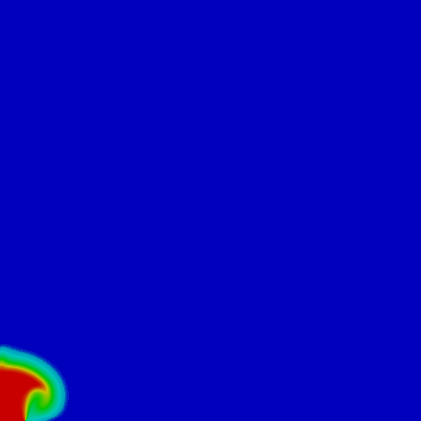
\includegraphics[width=0.32\columnwidth]{images/eruption_vfrac_10s.png}\hspace*{0.5mm}
      \centering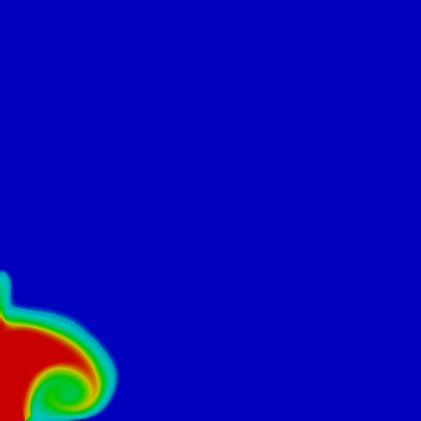
\includegraphics[width=0.32\columnwidth]{images/eruption_vfrac_30s.png}\hspace*{0.5mm}
      \centering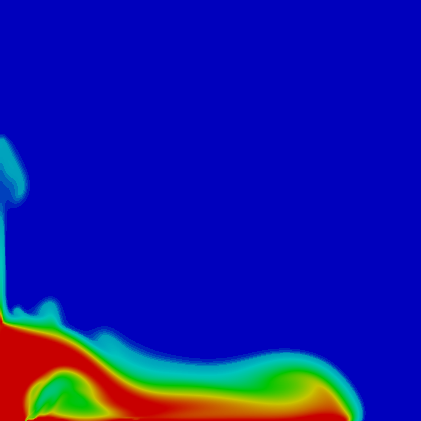
\includegraphics[width=0.32\columnwidth]{images/eruption_vfrac_70s.png}
      
      \centering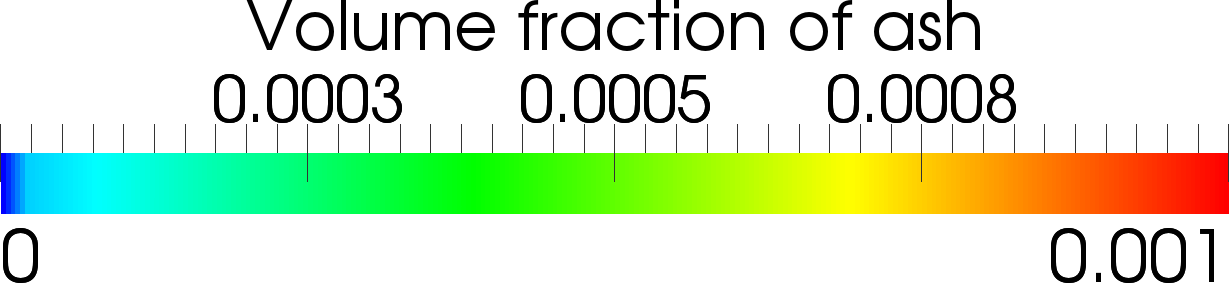
\includegraphics[width=0.3\columnwidth]{images/vfrac_legend.png}
   \end{figure}
}


\frame{
   \frametitle{What is data?}
   \framesubtitle{More examples} 
   Metadata from \texttt{www.firedrakeproject.org}
   \begin{figure}[H]
      \centering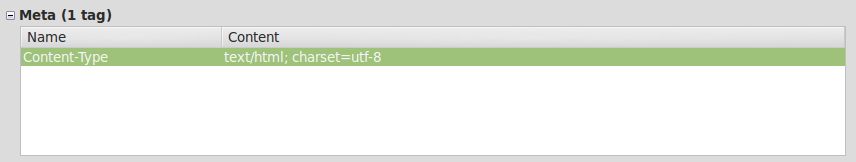
\includegraphics[width=0.9\columnwidth]{images/firedrakeproject_webpage_metadata.png}
   \end{figure}
}

\frame{
   \frametitle{What is data?}
   \framesubtitle{More examples} 
   Numerical solution error against grid spacing:
   \begin{figure}[H]
      \centering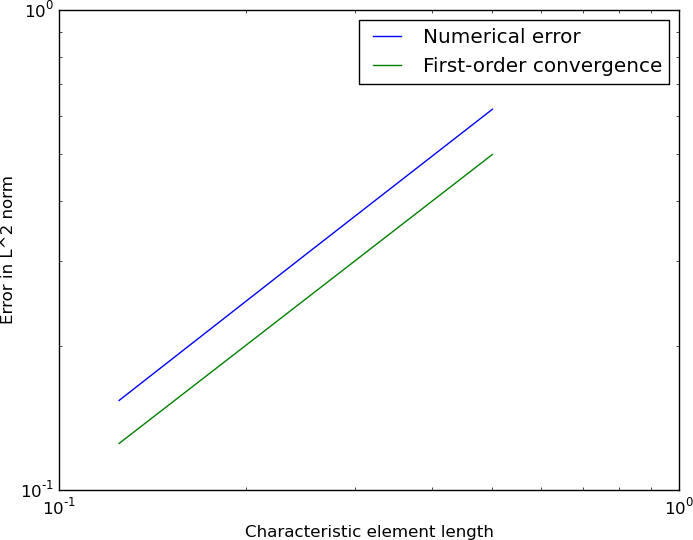
\includegraphics[width=0.7\columnwidth]{images/les_convergence.png}
   \end{figure}
}


\frame{
   \frametitle{Why is data important?}
   %\framesubtitle{Definition} 
   \begin{itemize}

    \item Allows {\color{red}new scientific discoveries} to be made.\vspace*{3mm}
    
    \item Journals and research councils are encouraging the {\color{red}sharing} of data to:
       \begin{itemize}
          \item promote research output,
          \item minimise the duplication of data,
          \item increase transparency and accountability, 
          \item allow fellow researchers to scrutinise and evaluate the data. 
       \end{itemize} \vspace*{3mm}
 
   \item The effective handling and management of all research data plays an important role in each of these processes. 
   
   \end{itemize}
}



\frame{
   \frametitle{Issues to consider}
   \framesubtitle{Data provenance} 
   \begin{itemize}
    \item {\color{red}Where} did the data originally come from? \vspace*{3mm}
    \item Can it be {\color{red}trusted}? (Are the authors known? Reputable journal?)
   \end{itemize}
}

\frame{
   \frametitle{Issues to consider}
   \framesubtitle{Licensing} 
   \begin{itemize}
    \item Who can use the data, and {\color{red}how}? Any user licence? \vspace*{3mm}
    \item Who owns the {\color{red}copyright}? Are you allowed to publish it or use it in your thesis?
    \begin{itemize}
      \item The Copyright Act allows for a certain degree of ``fair use''.
    \end{itemize}
    \vspace*{3mm}
    \item Creative Commons licences offer more open alternatives.
   \end{itemize}
}

\frame{
   \frametitle{Issues to consider}
   \framesubtitle{File formats} 
   \begin{itemize}
    \item Using {\color{red}standardised, open-source} file formats makes your data {\color{red}portable} and facilitates sharing of data by other researchers.  \vspace*{3mm}
    \item Comma-Separated Value ({\color{red}CSV}): a commonly-used format for simple data sets. Values in a single row are separated by commas. CSV files can contain multiple rows, thereby forming a table. \vspace*{3mm}
    \item eXtendable Markup Language ({\color{red}XML}): each piece of data has an element/tag and a value.
   \end{itemize}
}

\frame{
   \frametitle{Issues to consider}
   \framesubtitle{Storage options}
   \begin{itemize}
    \item Optical media (CDs ~700 MB, DVDs ~4.7 GB, Blu-ray 25+ GB) and flash drives - for small files e.g. presentations, theses, papers.\vspace*{3mm}
    \item Magnetic media (hard drives) - for larger files (e.g. simulation output).\vspace*{3mm}
    \item Cloud services.\vspace*{3mm}
    \item Always maintain a good {\color{red}file hierarchy} and {\color{red}naming convention} when storing data files.
   \end{itemize}
}

\frame{
   \frametitle{Issues to consider}
   \framesubtitle{Encryption}
   \begin{itemize}
    \item Be aware of responsibilities to encrypt sensitive information.\vspace*{3mm}
    \item Encrypting emails: Pretty Good Privacy (PGP) keys.\vspace*{3mm}
    \item Encrypting hard drives: \texttt{encryptfs} (Linux).
   \end{itemize}
}

\frame{
   \frametitle{Issues to consider}
   \framesubtitle{Backing up}
   \begin{itemize}
    \item \textbf{The importance of regularly backing up data cannot be stressed enough!}\vspace*{3mm}
    \item What if your hard drive failed right now? What if your computer was stolen?\vspace*{3mm}
    \item Storage space is reasonably cheap.\vspace*{3mm}
    \item Always keep {\color{red}several regular backups}, far apart from each other (not in the same building).\vspace*{3mm}
    \item Know the Imperial College data backup policy.
   \end{itemize}
}

\frame{
   \frametitle{Issues to consider}
   \framesubtitle{Big Data}
   \begin{itemize}
    \item {\color{red}Big Data} is one of the key challenges in data science.\vspace*{3mm}
    \item Involves data sets that are {\color{red}extremely large}, thereby creating additional difficulties when analysing them.\vspace*{3mm}
    \item Need novel and efficient tools to help tackle this issue.
   \end{itemize}
}

\end{document}
